\rchapter{Poisson Equation}

\section{Introduction}

Plasma is quasi-neutral. This means that although locally there may be charged regions, it is neutral overall. This condition is expressed by a Poisson equation. It is therefore important to have a robust and accurate method for solving Poisson equations in order to determine the electric potential.

The independence of the equations in the z-direction will be used to solve multiple equations in parallel. In addition, the method will use Fourier transforms to exploit the periodicity of the solution in the $\theta$-direction in order to obtain further parallelisation.

\section{Quasi-Neutrality Equation}

% \begin{equation}\label{quasi neutrality}
%  -\left[\partial_r^2\phi + \left(\frac{1}{r}+\frac{\partial_rn_0}{n_0}\right)\partial_r\phi+\frac{1}{r^2}\partial_\theta^2\phi\right]+\frac{1}{T_e(r)}\phi=\frac{1}{n_0}\int_{-\infty}^{+\infty}(f-f_{eq})dv_\parallel
% \end{equation}

As discussed in chapter \ref{chapter::Gyrokinetics}, the quasi-neutrality condition can be expressed using the following equation:

\begin{equation}\label{eq::quasi neutrality start}
 -\grad_\perp\cdot\left[\frac{\rho_{m0}}{\varepsilon_0B^2}\grad_\perp\phi\right]+\frac{1}{\lambda_D^2}\left[\phi-\chi\cdot\langle\phi\rangle_f\right]=\frac{1}{\varepsilon_0}\rho_{c1}
\end{equation}

where $\grad_\perp = \left(\grad-\hat{b}\left(\hat{b}\cdot\grad\right)\right)$, $\hat{b}$ is the magnetic unit vector as defined in equation \ref{eq::magnetic unit}, $\rho_{m0}$ is the equilibrium mass density, $\varepsilon_0$ is the permittivity of free space, $B$ is the intensity of the equilibrium background magnetic field, $\phi$ is the electrostatic potential, $\lambda_D$ is the electron Debye length, $\langle\phi\rangle_f$ is the flux-surface average of $\phi$, and $\rho_{c1}$ is the charge perturbation density due to the ions.

As discussed previously, for a torus to be effectively approximated by a straight cylinder, the major radius must be very large. As a result we let $\zeta(r)$ tend to 0. In this limit $\hat{b}$ tends towards $\hat{z}$. This means that the perpendicular gradient can be defined as follows:
\begin{align}
 \grad_\perp\phi=\grad\phi-\hat{b}\left(\hat{b}\cdot\grad\phi\right) \rightarrow& \grad\phi-\hat{z}\left(\hat{z}\cdot\grad\phi\right)\nonumber\\
 =&\partial_r\phi\hat{r}+\frac{1}{r}\partial_\theta\phi\hat{\theta}+\partial_z\phi\hat{z}-\partial_z\phi\hat{z}\nonumber\\
 =& \partial_r\phi\hat{r}+\frac{1}{r}\partial_\theta\phi\hat{\theta}
\end{align}

Defining $g(r)=\frac{\rho_{m0}(r)}{\varepsilon_0B^2}$, the first term in equation \ref{eq::quasi neutrality start} can now be expressed:
\begin{align}
\grad_\perp\left(g\grad_\perp\phi\right)=&\left(\grad-\hat{b}\left(\hat{b}\cdot\grad\right)\right)\cdot\left[g \grad \phi\right]\nonumber\\
\rightarrow& \left(\grad-\hat{z}\left(\hat{z}\cdot\grad\right)\right)\cdot\left[g \partial_r\phi\hat{r}+\frac{g}{r}\partial_\theta\phi\hat{\theta}\right]\nonumber\\
=&\frac{1}{r}\partial_r(rg\partial_r\phi)+\frac{1}{r}\partial_\theta(\frac{g}{r}\partial_\theta\phi)\nonumber\\
=&\frac{g}{r}\partial_r\phi+\partial_r(g\partial_r\phi)+\frac{g}{r^2}\partial_\theta^2\phi\nonumber\\
=&\frac{g}{r}\partial_r\phi+\partial_rg\partial_r\phi+g\partial_r^2\phi+\frac{g}{r^2}\partial_\theta^2\phi)\label{eq::grad perp sq}
\end{align}

Substituting equation \ref{eq::grad perp sq} and the definition of the charge perturbation density due to the ions into equation \ref{eq::quasi neutrality start} and dividing by g then leaves us with the following equation:
\begin{equation}\label{quasi neutrality}
 -\left[\partial_r^2+\left(\frac{1}{r}+\frac{\partial_rg}{g}\right)\partial_r+\frac{1}{r^2}\partial_\theta^2\right]\phi+\frac{1}{g\lambda_D^2}\left[\phi-\chi\cdot\langle\phi\rangle_\theta\right]=\frac{1}{g\varepsilon_0}\rho_{c1}
\end{equation}
where $\rho_{c1}=q_i\int (f-f_{eq})dv$ is the charge perturbation density due to the kinetic species.

This provides a simple differential equation which will be solved using the methods detailed in this chapter.

\section{Fourier Transform}

Fourier transforms decompose functions into the frequencies of which they are composed. This makes them practical for analysing periodic functions. The Fourier transform of a function is defined as followed:

\begin{equation}
 \hat{f}(k)=\mathcal{F}\left[f(x)\right]=\int_{-\infty}^{\infty}f(x)e^{-i k x}dx
\end{equation}

while the inverse Fourier transform is defined as follows:

\begin{equation}
 f(x)=\mathcal{F}^{-1}\left[\hat{f}(k)\right]=\int_{-\infty}^{\infty}\hat{f}(k)e^{i k x}dk
\end{equation}

In addition Fourier transforms have several useful properties. Notably the Fourier transform of a derivative is defined as follows:

$$\widehat{\frac{df}{dx}}(k)=i k \hat{f}(k)$$

The proof of this is shown below:

\begin{align*}
 \widehat{\frac{df}{dx}}(k)&=\mathcal{F}^{-1}\left[\frac{d}{dx}\int_{-\infty}^{\infty}\hat{f}(k)e^{i k x}dx\right]\\
 &=\mathcal{F}^{-1}\left[\int_{-\infty}^{\infty}\hat{f}(k)\frac{d}{dx}e^{i k x}dx\right]\\
 &=\mathcal{F}^{-1}\left[\int_{-\infty}^{\infty}\hat{f}(k)i k e^{i k x}dx\right]\\
 &=i k \hat{f}(k)
\end{align*}

This along with the linearity of the Fourier transform allows equation \ref{quasi neutrality} to be rewritten as follows:

\begin{align*}
 &\mathcal{F}_\theta\left[-\left[\partial_r^2+\left(\frac{1}{r}+\frac{\partial_rg}{g}\right)\partial_r\phi+\frac{1}{r^2}\partial_\theta^2\right]\phi+\frac{1}{g\lambda_D^2}\left[\phi-\chi\cdot\langle\phi\rangle_\theta\right]\right]\\
 =&-\partial_r^2\mathcal{F}_\theta\left[\phi\right] - \left(\frac{1}{r}+\frac{\partial_rg}{g}\right)\partial_r\mathcal{F}_\theta\left[\phi\right]-\frac{1}{r^2}(ik)^2\mathcal{F}_\theta\left[\phi\right]+\frac{1}{g\lambda_D^2}\left[\mathcal{F}_\theta\left[\phi\right]-\chi\delta_{k0}\mathcal{F}_\theta\left[\phi\right]\right]\\
 =&-\partial_r^2\mathcal{F}_\theta\left[\phi\right] - \left(\frac{1}{r}+\frac{\partial_rg}{g}\right)\partial_r\mathcal{F}_\theta\left[\phi\right]+\frac{k^2}{r^2}\mathcal{F}_\theta\left[\phi\right]+\frac{1}{g\lambda_D^2}\left[\mathcal{F}_\theta\left[\phi\right]-\chi\delta_{k0}\mathcal{F}_\theta\left[\phi\right]\right]\\
 =&\frac{1}{g\varepsilon_0}\mathcal{F}_\theta\left[\rho_{c1}\right]
\end{align*}

This leaves us with the following simplified equation which is a one-dimensional differential equation which can be solved using the finite elements method:
\begin{equation}\label{eq::quasi neutrality fourier}
 \left[-\partial_r^2 - \left(\frac{1}{r}+\frac{\partial_rg}{g}\right)\partial_r+\frac{k^2}{r^2}+\frac{1}{g\lambda_D^2}(1-\chi\delta_{k0})\right] \hat{\phi}=\frac{\hat{\rho}}{g\varepsilon_0}
\end{equation}

\section{Finite Elements}\label{sec::FE}

The finite elements method is a numerical method for solving various equations including Poisson equations. It consists of using the representation of functions on a given basis to formulate a matrix equation which can be solved to find the solution to the original equation.

All functions can be represented exactly on an infinite basis however this approach clearly doesn't work in a numerical setting. Instead the solution will be restricted to a subset of functions, with the finite elements method allowing the best approximation in this subset to be found. In this project the basis used will be B-Splines (see section \ref{sec::BSplines}). For a given mode $m$ and a given value of the $z$ coordinate, the solution can therefore be expressed as follows:
\begin{equation}\label{eq::FE discretisation}
\hat{\phi}(r,m,z)=\somme{i=0}{N}c_i\varphi_{i,m,z}(r)
\end{equation}

where $\varphi_{i,m,z}(r)$ is the i-th B-Spline basis for the values of the m and $z$ coordinates, and $c_i$ is the associated coefficient.

The weak form of an equation consists of multiplying it by a test function and integrating over the relevant domain. Any function satisfying the original equation should also satisfy the weak form of the equation for all test functions. If the test functions are chosen such that they form the basis of a function space then the equation stands for any test function in the function space. For this reason the test functions are often chosen to be the basis of the function space on which the solution is approximated.

The weak form of equation \ref{eq::quasi neutrality fourier} is shown below:
\begin{align}
 -\int_\Omega\partial_r^2\hat{\phi}(r,m)\,\psi(r) r\, dr & \nonumber\\
 - \int_\Omega\left(\frac{1}{r}+\frac{\partial_rg(r)}{g(r)}\right) \partial_r\hat{\phi}(r,m)\,\psi(r) r\, dr & \nonumber\\
 + \int_\Omega\left(\frac{k^2}{r^2}+\frac{1}{g(r)\lambda_D(r)^2}(1-\chi\delta_{k0})\right)\hat{\phi}(r,m)\,\psi(r) r\, dr&=\int_\Omega\frac{\hat{\rho}(r,m)}{g\varepsilon_0}\,\psi(r) r\, dr \label{quasi neutrality weak}
\end{align}
where $\Omega$ is the relevant domain, namely $[r_{min},r_{max}]$, $\psi(r)$ is the test function, and $r$ appears in the integral due to the Jacobian of the cylindrical coordinates.

The first term of this equation can be re-expressed as follows:
\begin{align}
 -\int_\Omega\partial_r^2\hat{\phi}(r,m)\,\psi(r)r\, dr =& \left.-\partial_r \hat{\phi}(r,m)\,\psi(r) r \right|_{\partial\Omega}+\int_\Omega\partial_r\hat{\phi}(r,m)\,\partial_r\psi(r)r\, dr\nonumber\\
 &+\int_\Omega\partial_r\hat{\phi}(r,m)\,\psi(r) dr\label{eq::FE boundary}
\end{align}

This avoids the use of high order derivatives which would decrease the accuracy of the solution. It also introduces a boundary term which allows the boundary conditions to be imposed.

In our simulations two types of boundary conditions will be used. These are homogeneous Dirichlet boundary conditions (where the boundary value is fixed at zero) and homogeneous Neumann boundary conditions (where the derivative at the boundary is fixed at zero). In the case of Neumann boundary conditions it is clear that the boundary term is equal to zero. In the case of Dirichlet boundary conditions the boundary term is also zero as long as the function space is restricted to functions which are also equal to zero on the boundary.

Inserting equation \ref{eq::FE boundary} and the basis representation described by equation \ref{eq::FE discretisation} into equation \ref{quasi neutrality weak} gives the following equation:
\begin{align}
 \underset{j}{\sum}\left[\int_\Omega\partial_r\varphi_j(r)\,\partial_r\psi_i(r)r\, dr \right. & \nonumber\\
 +\int_\Omega\partial_r\varphi_j(r)\,\psi_i(r) dr & \nonumber\\
 - \int_\Omega \left(\frac{1}{r}+\frac{\partial_rg(r)}{g(r)}\right)\partial_r\varphi_j(r)\,\psi_i(r)r\, dr & \\
 \left.+ \int_\Omega\left(\frac{k^2}{r^2}+\frac{1}{g(r)\lambda_D(r)^2}(1-\chi\delta_{k0})\right)\varphi_j(r)\,\psi_i(r)r\, dr\right]&c_j=\int_\Omega\frac{\hat{\rho}(r,m)}{g(r)\varepsilon_0}\,\psi_i(r)r\, dr\nonumber
\end{align}

The solution to the problem is therefore the coefficients $c_j$. Everything else can be expressed using the definitions of the B-Splines and a quadrature scheme. The quadrature scheme used in this project is Gauss-Legendre quadrature which is exact for polynomials of degree 2n-1 when n is the number of different points required to calculate the quadrature. This equation can also be expressed in matrix notation, in this case the integral is contained within a matrix $\mat{A}\in\reel^{N\text{x}N}$, known as the stiffness matrix, and defined as follows:
\begin{align}
 \mat{A}_{ij}=&\int_\Omega\partial_r\varphi_j(r)\,\partial_r\psi_i(r)r\, dr +\int_\Omega\partial_r\varphi_j(r)\,\psi_i(r) dr\nonumber\\
 &- \int_\Omega\left(\frac{1}{r}+\frac{\partial_rg(r)}{g(r)}\right) \partial_r\varphi_j(r)\,\psi_i(r)r\, dr\nonumber\\
 &+ \int_\Omega\left(\frac{k^2}{r^2}+\frac{1}{g(r)\lambda_D(r)^2}(1-\chi\delta_{k0})\right)\varphi_j(r)\,\psi_i(r)r\, dr
\end{align}

The right-hand side is a vector $\vec{b}\in\reel^{N}$:
\begin{equation}
 \vec{b}_i = \int_\Omega\frac{\hat{\rho}(r,m)}{g(r)\varepsilon_0}\,\psi_i(r)r\, dr\nonumber
\end{equation}

As mentioned previously $\hat{\rho}$ is the Fourier transform of $\rho_{c1}$ which is defined as follows:
\begin{equation}
 \rho_{c1} = q_i \int (f - f_{eq}) dv
\end{equation}

The values will therefore be calculated at each point for which the value of the distribution function $f$ is stored. These points are the Greville points of a spline function. The result is therefore an approximation of $\hat{\rho}$ in the function space of the splines. As a result it can also be expressed using b-splines:
\begin{equation}\label{eq::rho discretisation}
\hat{\rho}(r,m,z)=\somme{i=0}{N}p_i\varphi_{i,m,z}(r)
\end{equation}

The vector $\vec{b}$ can therefore be rewritten as:
\begin{equation*}
 \vec{b}_i = \underset{j}{\sum}p_j\int_\Omega\frac{1}{g(r)\varepsilon_0} \psi_j(r) \,\psi_i(r)r\, dr
\end{equation*}

The vector can therefore also be expressed in matrix notation. In this case the integral is contained within a matrix $\mat{M}\in\reel^{N\text{x}N}$, known as the mass matrix, and defined as follows:
\begin{equation}
 M_{ij}=\int_\Omega\frac{1}{g(r)\varepsilon_0} \psi_j(r) \,\psi_i(r)r\, dr
\end{equation}


The coefficients $c_j$ are therefore the elements of the vector $\vec{c}\in\reel^N$, solution of the matrix equation $\mat{A}\vec{c}=\mat{M}\vec{p}$

\section{B-Spline}\label{sec::BSplines}

B-splines are a basis of the function space containing splines. A spline $s(x)$ is a piece-wise polynomial function. It is defined by a degree d, and knots $x_0,\dots,x_m$ such that $a_i\leq a_{i+1}$ and $s(x)$ is (d-r) times differentiable at any knot which appears r times\cite{SplineBook}. In this project, the knots for n-th degree splines will always be chosen such that the spline is $\mathcal{C}^{d-1}$. This means that repeated knots can only appear on the boundary of the considered domain.

Every function space can have multiple different bases. B-splines are a specific basis defined as follows:
\begin{gather}
 N_i^0(x)=
 \begin{cases}
  1\quad\quad \text{ if } x\in[x_i,x_{i+1}[\\
  0\quad\quad \text{ otherwise}
 \end{cases}\\
 N_i^{n} = \alpha_i^{n-1}N_i^{n-1}(x)+\left(1-\alpha_{i+1}^{n-1}\right)N_{i+1}^{n-1}(x)\\
 \alpha_i^{n-1}=
 \begin{cases}
  \frac{u-x_i}{x_{i+n}-x_i}\quad\quad \text{ if } x_{i+n}\neq x_i\\
  0\quad\quad\quad \text{ otherwise}
 \end{cases}
\end{gather}

The b-spline basis for 3-rd degree splines can be seen in figure \ref{3rd degree BSplines}. Note that the central splines cover d+1=4 elements $[a_i,a_{i+1}[$. Therefore d+2 knots are required for each basis function. The additional knots required for the functions nearer to the edge of the domain are repeated knots on the boundary; thus $a_0=a_1=\dots=a_d$, and $a_m=a_{m-1}=\dots=a_{m-d}$.

\begin{figure}[ht]
 \centering
 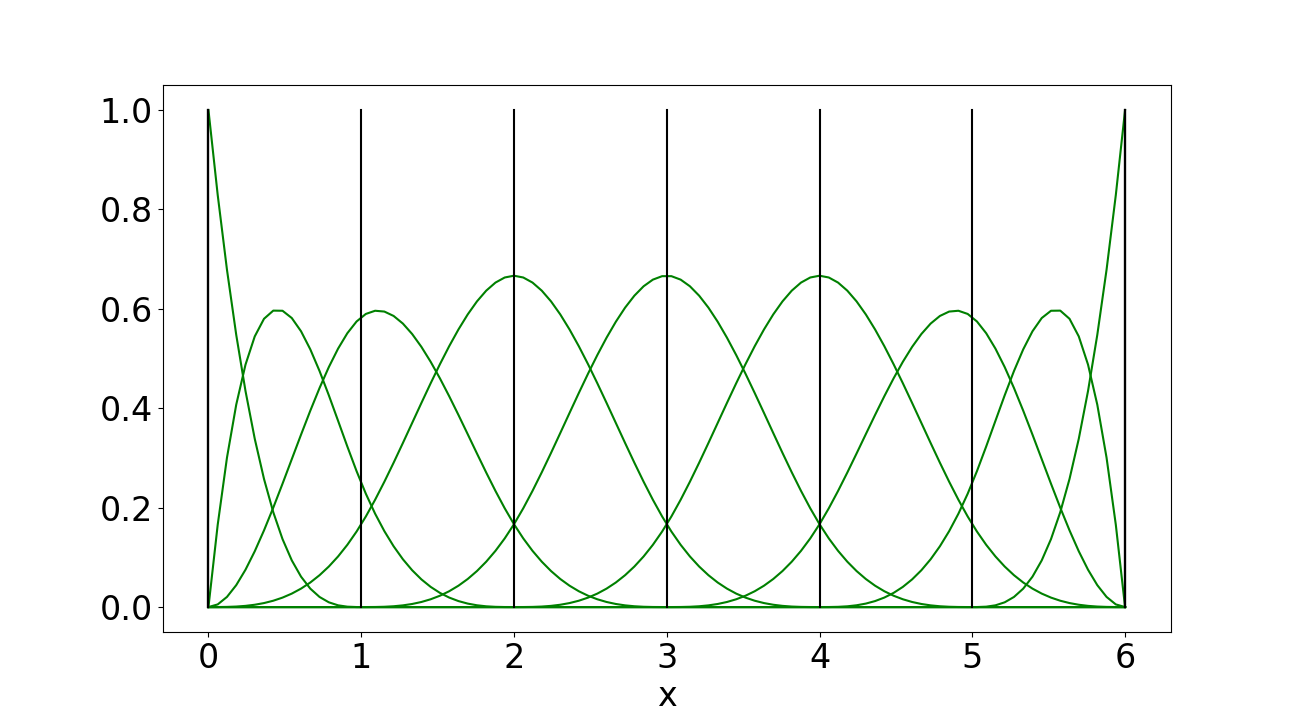
\includegraphics[width=\textwidth]{Figs/bSplines.png}
 \caption{\label{3rd degree BSplines}3rd degree B-Spline with additional knots found on the boundary}
\end{figure}

The d-th degree splines, which make up the function space to which the solution of the Finite Elements problem will belong, can therefore be expressed as follows:
\begin{align}
s(x)=\underset{i}{\sum}c_iN_i^d(x)
\end{align}

The shape of the B-Splines therefore means that the mass and stiffness matrices will be band matrices.

\section{Implementation Details}

The aforementioned schemes will therefore be used to implement equation \ref{quasi neutrality}:
\begin{equation}
 -\left[\partial_r^2+\left(\frac{1}{r}+\frac{\partial_rg}{g}\right)\partial_r+\frac{1}{r^2}\partial_\theta^2\right]\phi+\frac{1}{g\lambda_D^2}\left[\phi-\chi\cdot\langle\phi\rangle_\theta\right]=\frac{1}{g\varepsilon_0}\rho_{c1}
\end{equation}

Note that $g\lambda_D^2=\frac{m\kappa T_e(r)}{B^2q_e^2}$, $\frac{\partial_rg}{g}=\frac{\partial_rn_0}{n_0}$ and $g\varepsilon_0=\frac{mn_0(r)}{B^2}$. For implementation purposes, it is supposed that m=q=1. Thus the following parameters must be provided to complete the problem:
\begin{itemize}
 \item $n_0(r)$
 \item $\partial_rn_0(r)$ (in practice $\frac{\partial_rn_0(r)}{n_0(r)}$ may be provided if it can be expressed more simply)
 \item $B$
 \item $\kappa T_e(r)$
 \item $\chi$
\end{itemize}

In addition an additional parameter will be requested in order to signify whether electrons are considered to be a kinetic or adiabatic species. In the kinetic case it will be assumed that $\frac{1}{\lambda_D^2}=0$.

The above equation is somewhat complicated and it is therefore preferable to implement the following equation:
\begin{equation}
 a\cdot\partial_r^2\phi+b\cdot\partial_r\phi+c\cdot\phi+d\cdot\partial_\theta^2\phi=e\cdot\rho
\end{equation}
where a is a constant and b,c,d and e are any functions dependant on r, in order to be able to test each element of the equation individually. This makes it easier to locate any errors in the scheme.

The following matrices will then be built:
\begin{gather}
 A_{ij}=\int_\Omega a\left(\partial_r\phi_j\partial_r\psi_i r + \partial_r\phi_j\psi_i\right)\, dr\\
 B_{ij}=\int_\Omega b(r)\partial_r\phi_j\psi_i r\, dr\\
 C_{ij}=\int_\Omega c(r)\phi_j\psi_i r\, dr\\
 D_{ij}=\int_\Omega d(r)\phi_j\psi_i r\, dr\\
 E_{ij}=\int_\Omega e(r)\phi_j\psi_i r\, dr
\end{gather}

The solution will therefore be the solution $\vec{\phi}$ to the following matrix equation:
\begin{equation}
 \left(-\mat{A}+\mat{B}+\mat{C}-k^2\mat{D}\right)\vec{\phi}=\mat{E}\vec{\rho}
\end{equation}

As mentioned in section \ref{sec::FE} Dirichlet and Neumann homogeneous boundary conditions will be used. Dirichlet boundary conditions will be imposed by restricting the function space of both the test functions and the solution. Specifically this is done by reducing the basis so that it no longer includes the function which is not zero at the boundary. This means that the solution is no longer expressed as in equation \ref{eq::FE discretisation}, but is instead expressed as follows:
\begin{equation}
\hat{\phi}(r,m,z)=\somme{i=1}{N-1}c_i\varphi_{i,m,z}(r)
\end{equation}

Care should be taken with this formulation as the right hand side is still expressed as in equation \ref{eq::rho discretisation}. This means that the mass matrix is a rectangular matrix.

The boundary conditions used at $r=r_\text{max}$ are always homogeneous Dirichlet conditions. At $r=r_\text{min}$ the boundary conditions are homogeneous Dirichlet conditions for all modes except the 0-th mode where homogeneous Neumann conditions are used.

\section{Convergence}

The convergence order of the scheme described above will be determined by testing the following equation:
\begin{equation}\label{eq::Convergence QN}
 \left[-\partial_{r}^2 - \left[\frac{1}{r} - \kappa_{n_0} \left(1 - \tanh\left( \frac{r - r_p }{\delta_{r_{n_0}}}\right)^2\right)\right]\partial_r + \frac{1}{T_e(r)}-\frac{1}{r^2}\partial_\theta^2\right]\phi = \rho
\end{equation}

The function $\rho$ will be determined by choosing a solution and substituting this into equation \ref{eq::Convergence QN}. The solution chosen will be the following:
\begin{equation}\label{eq::Convergence QN solution}
 \phi(r,\theta)=\cos\left(\frac{3\pi(r-r_{\min})}{2(r_{\max}-r_{\min})}\right)^4\sin(\theta)^3
\end{equation}

The boundary conditions will be Neumann at $r=r_{\min}$ and Dirichlet at $r=r_{\max}$. This solution can be seen in figure \ref{fig::Convergence QN shape}.

Tests have shown that the Fourier transform is exact to machine precision for this function even for small values of $N_\theta$. The results therefore show only the convergence as a function of the number of finite elements in the $r$ direction. We expect that a convergence order of d+1 when splines of degree d are used.

\begin{figure}[b!]
 \centering
 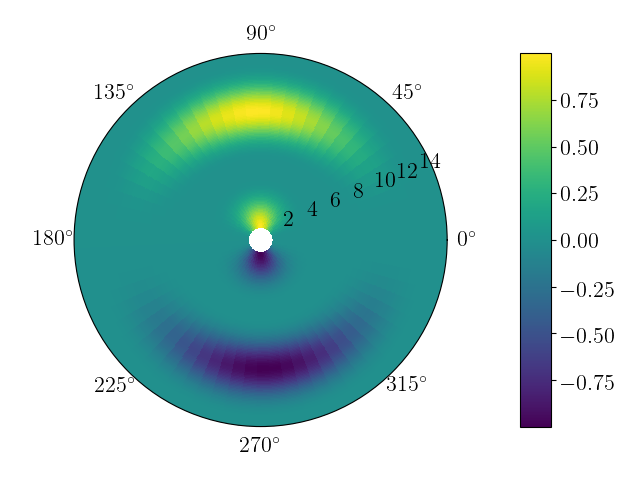
\includegraphics[width=.7\textwidth]{Figs/PoissonConvergence/ExactSolution.png}
 \caption{\label{fig::Convergence QN shape} The form of equation \ref{eq::Convergence QN solution}, the chosen solution of equation \ref{eq::Convergence QN} used to test convergence. $N_r=128$, $N_\theta=64$}
\end{figure}

\begin{table}[p]
 \begin{tabular}{|r c|r c|c|c|c|c|}
 \hline
 \multicolumn{2}{|c|}{\bf Spline} & \multicolumn{2}{|c|}{\bf N$_\text{elem}$} & \bf L$^2$ norm       & \bf Order & \bf L$^\infty$ norm  & \bf Order\\
 \multicolumn{2}{|c|}{\bf degree} &  & &        &  &   & \\
 \hline
 \hline
1  & &  16     & & $ 1.27 \cdot 10^{ -1 }$ &       & $ 4.59 \cdot 10^{ -2 }$ &  \\
\hline
1  & &  32     & & $ 3.28 \cdot 10^{ -2 }$ &  1.95  & $ 1.43 \cdot 10^{ -2 }$ &  1.69  \\
\hline
1  & &  64     & & $ 8.28 \cdot 10^{ -3 }$ &  1.99  & $ 3.91 \cdot 10^{ -3 }$ &  1.87  \\
\hline
1  & &  128     & & $ 2.08 \cdot 10^{ -3 }$ &  2.00  & $ 1.01 \cdot 10^{ -3 }$ &  1.95  \\
\hline
1  & &  256     & & $ 5.19 \cdot 10^{ -4 }$ &  2.00  & $ 2.56 \cdot 10^{ -4 }$ &  1.98  \\
\hline
1  & &  512     & & $ 1.30 \cdot 10^{ -4 }$ &  2.00  & $ 6.44 \cdot 10^{ -5 }$ &  1.99  \\
\hline
1  & &  1024     & & $ 3.25 \cdot 10^{ -5 }$ &  2.00  & $ 1.61 \cdot 10^{ -5 }$ &  2.00  \\
\hline
1  & &  2048     & & $ 8.12 \cdot 10^{ -6 }$ &  2.00  & $ 4.03 \cdot 10^{ -6 }$ &  2.00  \\
\hline
 \hline
2  & &  16     & & $ 9.98 \cdot 10^{ -3 }$ &       & $ 7.40 \cdot 10^{ -3 }$ &  \\
\hline
2  & &  32     & & $ 9.56 \cdot 10^{ -4 }$ &  3.38  & $ 8.11 \cdot 10^{ -4 }$ &  3.19  \\
\hline
2  & &  64     & & $ 9.30 \cdot 10^{ -5 }$ &  3.36  & $ 6.92 \cdot 10^{ -5 }$ &  3.55  \\
\hline
2  & &  128     & & $ 9.41 \cdot 10^{ -6 }$ &  3.30  & $ 5.75 \cdot 10^{ -6 }$ &  3.59  \\
\hline
2  & &  256     & & $ 1.05 \cdot 10^{ -6 }$ &  3.16  & $ 5.45 \cdot 10^{ -7 }$ &  3.40  \\
\hline
2  & &  512     & & $ 1.26 \cdot 10^{ -7 }$ &  3.06  & $ 6.02 \cdot 10^{ -8 }$ &  3.18  \\
\hline
2  & &  1024     & & $ 1.56 \cdot 10^{ -8 }$ &  3.02  & $ 7.09 \cdot 10^{ -9 }$ &  3.09  \\
\hline
2  & &  2048     & & $ 1.94 \cdot 10^{ -9 }$ &  3.00  & $ 8.60 \cdot 10^{ -10 }$ &  3.04  \\
\hline
 \hline
3  & &  16     & & $ 2.38 \cdot 10^{ -3 }$ &       & $ 8.76 \cdot 10^{ -4 }$ &  \\
\hline
3  & &  32     & & $ 2.00 \cdot 10^{ -4 }$ &  3.57  & $ 1.51 \cdot 10^{ -4 }$ &  2.54  \\
\hline
3  & &  64     & & $ 2.50 \cdot 10^{ -5 }$ &  3.00  & $ 2.21 \cdot 10^{ -5 }$ &  2.77  \\
\hline
3  & &  128     & & $ 2.30 \cdot 10^{ -6 }$ &  3.45  & $ 2.20 \cdot 10^{ -6 }$ &  3.33  \\
\hline
3  & &  256     & & $ 1.74 \cdot 10^{ -7 }$ &  3.73  & $ 1.75 \cdot 10^{ -7 }$ &  3.65  \\
\hline
3  & &  512     & & $ 1.19 \cdot 10^{ -8 }$ &  3.87  & $ 1.24 \cdot 10^{ -8 }$ &  3.82  \\
\hline
3  & &  1024     & & $ 7.78 \cdot 10^{ -10 }$ &  3.93  & $ 8.23 \cdot 10^{ -10 }$ &  3.91  \\
\hline
3  & &  2048     & & $ 4.99 \cdot 10^{ -11 }$ &  3.96  & $ 5.32 \cdot 10^{ -11 }$ &  3.95  \\
\hline
 \hline
4  & &  16     & & $ 4.41 \cdot 10^{ -4 }$ &       & $ 1.76 \cdot 10^{ -4 }$ &  \\
\hline
4  & &  32     & & $ 1.88 \cdot 10^{ -5 }$ &  4.55  & $ 1.61 \cdot 10^{ -5 }$ &  3.45  \\
\hline
4  & &  64     & & $ 1.04 \cdot 10^{ -6 }$ &  4.18  & $ 9.28 \cdot 10^{ -7 }$ &  4.12  \\
\hline
4  & &  128     & & $ 3.45 \cdot 10^{ -8 }$ &  4.91  & $ 3.19 \cdot 10^{ -8 }$ &  4.86  \\
\hline
4  & &  256     & & $ 8.17 \cdot 10^{ -10 }$ &  5.40  & $ 7.63 \cdot 10^{ -10 }$ &  5.38  \\
\hline
4  & &  512     & & $ 1.62 \cdot 10^{ -11 }$ &  5.66  & $ 1.53 \cdot 10^{ -11 }$ &  5.64  \\
\hline
4  & &  1024     & & $ 3.00 \cdot 10^{ -13 }$ &  5.75  & $ 2.79 \cdot 10^{ -13 }$ &  5.78  \\
\hline
 \end{tabular}
\caption{\label{tab::Convergence QN} Convergence of the Finite Elements method for equation \ref{eq::Convergence QN} with $N_\theta=8$}
\end{table}

The results are shown in table \ref{tab::Convergence QN}, and figure \ref{fig::Convergence QN}. It can be seen that the 1st degree spline approximation converges with the expected order, while the 2nd and 3rd degree spline approximations converge to the correct order. The 4th degree spline approximation has approximately the correct order however it is hard to gain conclusive evidence as the error quickly approaches machine precision which causes errors which are not due to the method.

\begin{figure}[h]
 \centering
 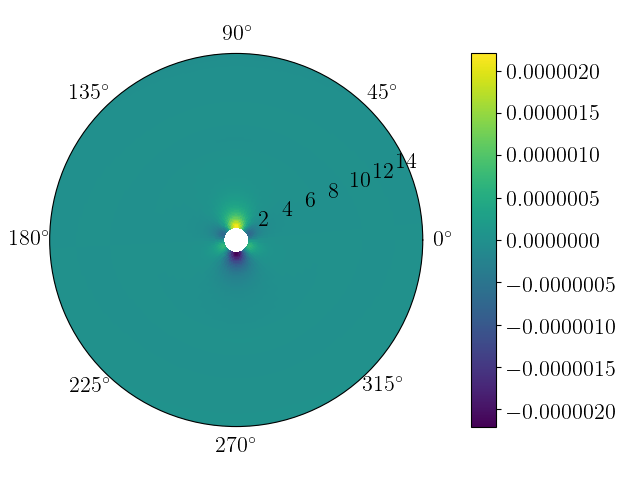
\includegraphics[width=.65\textwidth]{Figs/PoissonConvergence/Error.png}
 \caption{\label{fig::Convergence QN Error} Error of the solution of equation \ref{eq::Convergence QN}, where the exact solution is specified by equation \ref{eq::Convergence QN solution}. Note that most errors are found near the Neumann boundary.}
\end{figure}

\begin{figure}[h]
 \centering
 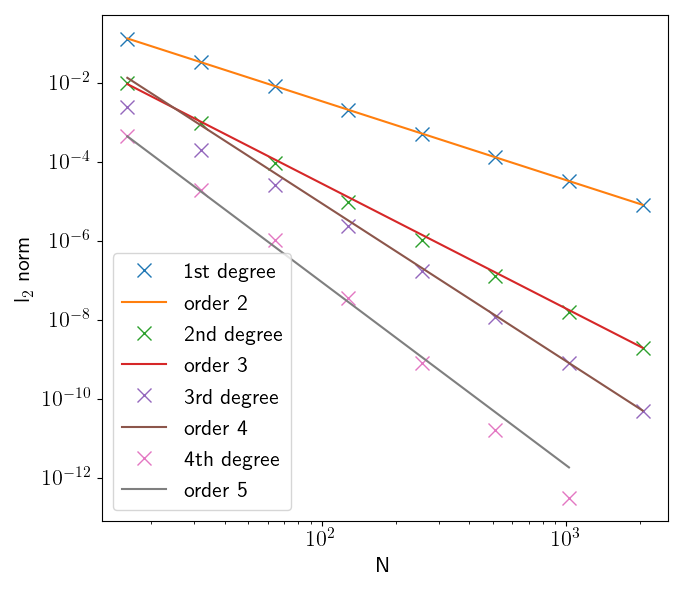
\includegraphics[width=.69\textwidth]{Figs/PoissonConvergence/l2_elementwise.png}
 \vspace{-1em}
 \caption{\label{fig::Convergence QN} Convergence of the Finite Elements method for equation \ref{eq::Convergence QN}. Exact values can be found in table \ref{tab::Convergence QN}}
\end{figure}
